% !TEX root = _individual/adDerivation.tex

%%%%%%%%%%%%%%%%%%%%%%%%%%%%%%%%%%%%%%%%%%%%%%%%%%%%%%%%%%%%%%%%%%%%%%%%%%%%%%%%
\chapter{Anisotropic diffusion}\label{chap:adDerivation}

The common radiation transport methods presented
in the last chapter approximate the angular dependence of the intensity each
in a different way. The crudest of these methods, diffusion, has only one
unknown
$\phi$ at each point in space and time; the more complex such as \SN\ have many
unknowns, leading to greater accuracy but greater computer run time and memory
usage. In this chapter, we derive a new anisotropic diffusion method which
approximates the intensity in such a way as to retain an arbitrary amount of
anisotropy (like a true transport method), while solving for a single unknown
(like a diffusion method).

The previous work in anisotropic diffusion has only considered steady-state,
linear problems in an infinite medium \cite{Lar2009c,Mor2007}. The novel work
presented in this chapter provides a
theoretical basis for using AD in time-dependent, nonlinear problems, and it
also addresses boundary conditions for the AD method.

%%%%%%%%%%%%%%%%%%%%%%%%%%%%%%%%%%%%%%%%%%%%%%%%%%%%%%%%%%%%%%%%%%%%%%%%%%%%%%%%
\section{Derivation}\label{sec:adDerivation}

In this section, we use an asymptotic analysis to derive the anisotropic
diffusion approximation in a linear, time-dependent, finite problem. We will
later demonstrate this analysis' applicability to nonlinear thermal radiative
transfer.

%\clearpage
The linear, time-dependent transport equation with isotropic scattering is
\begin{subequations} \label{eqs:tdTransport}
\begin{multline} \label{eq:tdTransportVol}
  \frac{1}{c}\pder{I}{t}(\vec{x},\vec{\Omega},t)
  + \vec{\Omega}\vd \grad I(\vec{x},\vec{\Omega},t)
  + \sigma(\vec{x}) I(\vec{x},\vec{\Omega},t)
  \\ = \frac{\sigma_s(\vec{x})}{4\pi}
  \int_{4\pi} I(\vec{x},\vec{\Omega}',t) \ud \Omega'
  + \frac{q(\vec{x},t)}{4\pi}
  \,, \quad \vec{x}\in V,\ \vec{\Omega}\in4\pi,\ t \ge 0.
\end{multline}
The boundary condition is specified
for incident directions:
\begin{equation} \label{eq:tdTransportBndy}
  I(\vec{x},\vec{\Omega},t) = I^b(\vec{x},\vec{\Omega},t) \,,
  \quad \vec{x}\in \partial V ,\ \vec{\Omega}\vd \vec{n} < 0,\ t > 0,
\end{equation}
and the initial condition is
\begin{equation} \label{eq:tdTransportInit}
  I(\vec{x},\vec{\Omega},0) = I^i(\vec{x},\vec{\Omega}) \,,
  \quad \vec{x}\in V ,\ \vec{\Omega} \in 4\pi.
\end{equation}
\end{subequations}
For consistency with the rest of this thesis, we retain the nomenclature of
radiative transfer rather than neutron transport.\footnote{
To enumerate the differences: we refer to
the ``radiative intensity'' $I$ rather than the ``angular flux'' $\psi$,
the ``scalar intensity'' rather than the ``scalar flux'',
the ``radiation flux'' $\vec{F}$ rather than the ``neutron current'' $\vec{J}$,
the ``opacity'' $\sigma$ rather than the ``total cross section'' $\Sigma_t$,
and so on.
}

Because this transport equation is linear, we can write its solution as the
linear superposition of three distinct transport solutions:
\begin{equation}\label{eq:tdSuperposition}
  I(\vec{x},\vec{\Omega},t)
  \equiv \Iv(\vec{x},\vec{\Omega},t)
  + \Ibl(\vec{x},\vec{\Omega},t)
  + \Iil(\vec{x},\vec{\Omega},t)\,.
\end{equation}
Here, $\Iv$ is an ``interior'' solution, valid several mean free paths away from
the exterior problem boundary and several free times away from $t=0$; $\Ibl$ is
a
``boundary layer'' solution that decays rapidly away from the exterior boundary;
and $\Iil$ is an ``initial layer'' that decays rapidly away from $t=0$.
Figure~\ref{fig:layers} represents these three regimes graphically. In the
interior, spatial and temporal variations are small; in the boundary layer,
spatial variations normal to the boundary are large; and in the initial layer,
the temporal variations are large.

\begin{figure}[htb]
  \centering
  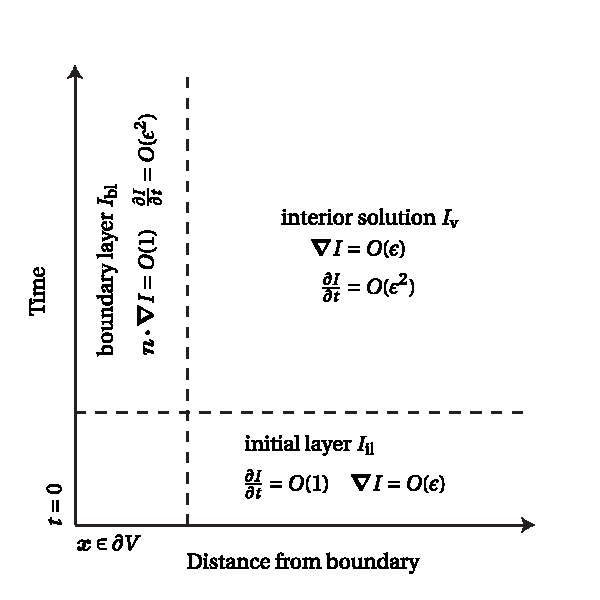
\includegraphics{layers}
  \caption{Depiction of interior, boundary layer, and initial layer of a
  transport problem.}
  \label{fig:layers}
\end{figure}

Our goal is first to develop an approximation to $\Iv$ that satisfies the transport
equation in some asymptotic limit, and then to use the boundary and initial layer
equations to ``match'' the interior solution to the transport solution on the
boundary and at the initial time. This procedure follows prior work in the
field, e.g.~the asymptotic derivation of the diffusion equation with
transport-matched boundary conditions \cite{Mal1991}.

%%%%%%%%%%%%%%%%%%%%%%%%%%%%%%%%%%%%%%%%%%%%%%%%%%%%%%%%%%%%%%%%%%%%%%%%%%%%%%%%
\subsection{Interior solution}\label{sec:adInterior}

The transport equation for the interior accounts for the extraneous source term,
but
it has no initial or boundary conditions, as it is only valid away from the
boundary and initial layer:
\begin{equation} \label{eq:tdVol}
  \frac{1}{c}\pder{\Iv}{t}(\vec{x},\vec{\Omega},t)
  + \vec{\Omega}\vd \grad \Iv(\vec{x},\vec{\Omega},t)
  + \sigma(\vec{x}) \Iv(\vec{x},\vec{\Omega},t)
  = \frac{\sigma_s(\vec{x})}{4\pi}
  \phi(\vec{x},t) + \frac{q(\vec{x},t)}{4\pi} \,.
\end{equation}
Here, we have defined
\begin{equation} \label{eq:tdPhi}
  \phi(\vec{x}) \equiv \int_{4\pi} \Iv(\vec{x}, \vec{\Omega},t) \ud \Omega\,,
\end{equation}
which is the \emph{interior} scalar intensity. We write Eq.~\eqref{eq:tdVol} as
\begin{equation*}
  \left[ \frac{1}{c}\pder{}{t}
  + \vec{\Omega}\vd \grad
  + \sigma \right] \Iv
  = \frac{\sigma_s}{4\pi}
  \phi + \frac{q}{4\pi} \,.
\end{equation*}

Taking the zeroth angular moment of Eq.~\eqref{eq:tdVol} gives a
\emph{conservation equation} in the interior,
\begin{equation} \label{eq:loVol}
\frac{1}{c} \pder{\phi}{t} (\vec{x}, t)
  + \grad \vd\vec{F}(\vec{x}, t)
  + \sigma(\vec{x}) \phi(\vec{x}, t)
 = \sigma_s(\vec{x}) \phi(\vec{x},t) + q(\vec{x},t)\,.
\end{equation}
Here we have defined the \emph{interior} radiation flux:
\begin{equation}\label{eq:tdF}
  \vec{F} \equiv \int_{4\pi} \vec{\Omega} \Iv(\vec{x}, \vec{\Omega},t) \ud
  \Omega\,,
\end{equation}
the first angular moment of the \emph{interior} solution.

Adding $\vec{\Omega}\vd \grad \phi$ to both sides of Eq.~\eqref{eq:loVol} and
multiplying the resulting equation by $\frac{1}{4\pi}$, we obtain
\begin{align*}
  \left[ \frac{1}{c}\pder{}{t}
  + \vec{\Omega}\vd \grad
  + \sigma \right]
  \left( \frac{1}{4\pi} \phi \right)
  = \frac{\sigma_s}{4\pi}
  \phi + \frac{q}{4\pi} - \frac{1}{4\pi} \grad \vd\vec{F} 
  + \frac{1}{4\pi} \vec{\Omega}\vd \grad \phi\,.
\end{align*}
Subtracting this equation from Eq.~\eqref{eq:tdVol} cancels the isotropic source
and scattering term on the right-hand side, yielding the following equation:
\begin{equation}\label{eq:capPsiVol}
  \left[ \frac{1}{c}\pder{}{t}
  + \vec{\Omega}\vd \grad
  + \sigma \right]
   \left( \Iv
  - \frac{1}{4\pi} \phi \right)
  = \frac{1}{4\pi} \grad \vd\vec{F} -
  \frac{1}{4\pi} \vec{\Omega}\vd \grad \phi\,.
\end{equation}

At this point, we apply an asymptotic scaling typical of a diffusive regime.
We make an ansatz that the spatial gradient of the solution is weak, the time
derivative is very small, and the solution is mildly (but not necessarily
linearly) anisotropic:
\begin{align} \label{eq:ansatz}
  \sigma &= O(1), &
  I &= O(1), &
  \int_{4\pi} \vec{\Omega} I \ud\Omega &= O(\epsilon), &
  \grad I &= O(\epsilon), &
  \pder{I}{t} &= O(\epsilon^2) \,.
\end{align}
These scalings are the same as in an asymptotic derivation of the standard
diffusion equation \cite{Lar1975,Mor2000}. With the scalings applied,
Eq.~\eqref{eq:capPsiVol} is written with the asymptotically small terms lumped
together:
\begin{equation*}
  \left[\vec{\Omega}\vd \grad
  + \sigma + O(\epsilon^2) \right]
   \left( \Iv
  - \frac{1}{4\pi} \phi \right)
  = - \frac{1}{4\pi} \vec{\Omega}\vd \grad \phi + O(\epsilon^2)\,.
\end{equation*}
Neglecting the high-order $O(\epsilon^2)$ terms, we make the first approximation
yet, obtaining:
\begin{equation}\label{eq:tdVolApprox1}
  \left[\vec{\Omega}\vd \grad  + \sigma \right]
   \left( \Iv
  - \frac{1}{4\pi} \phi \right)
  = - \frac{1}{4\pi} \vec{\Omega}\vd \grad \phi \,.
\end{equation}
Formally inverting the bracketed operator on the left-hand side, we obtain an
approximate expression for the intensity in the interior:
\begin{equation}\label{eq:tdVolApprox2}
  \Iv = \frac{1}{4\pi} \phi - 
  \left[\vec{\Omega}\vd \grad  + \sigma \right]\inv
  \left( \frac{1}{4\pi} \vec{\Omega}\vd \grad \phi \right)\,.
\end{equation}

The inverted differential operator is an integral transport operator
\cite{Pri2010}:
\begin{subequations} \label{eqs:inverseTransport}
  \begin{align} \label{eq:inverseTransportFull}
  \begin{split}
    \left[\vec{\Omega}\vd \grad  + \sigma \right]\inv
    \hat Q(\vec{x}, \vec{\Omega},t)
    &=
     \int_{0}^{\infty}
    \hat Q(\vec{x} - s \vec{\Omega}, \vec{\Omega}, t)
    \eexp^{ -\tau(\vec{x}, \vec{x} - s \vec{\Omega})}
    \ud s
\,.
  \end{split}
  \end{align}
  Here we have used the optical distance between points $\vec{x}$ and
  $\vec{x}'$ along the direction $\vec{\Omega} = (\vec{x}'-
  \vec{x})/\norm{\vec{x}'-\vec{x}}$:
  \begin{equation} \label{eq:fullTauDefinition}
    \tau(\vec{x}, \vec{x}') = \int_{0}^{\norm{\vec{x} -
    \vec{x}'}} \sigma(\vec{x}-s\vec{\Omega}) \ud s \,.
  \end{equation}
\end{subequations}

Thus Eq.~\eqref{eq:tdVolApprox2} for the interior intensity is a function of the
nonlocal, unknown scalar intensity:
\begin{equation}\label{eq:tdVolApprox1a}
  \Iv(\vec{x},\vec{\Omega},t) = \frac{1}{4\pi} \phi(\vec{x},t) - 
     \int_{0}^{\infty}
    \frac{1}{4\pi} \vec{\Omega}\vd \grad \phi(\vec{x} - s \vec{\Omega}, \vec{\Omega}, t)
    \eexp^{ -\tau(\vec{x}, \vec{x} - s \vec{\Omega})}
    \ud s \,.
\end{equation}
To simplify, we use the assumption from Eq.~\eqref{eq:ansatz} that spatial
gradients are weak to expand $\phi$ in a Taylor series about the local
point:
\begin{equation} \label{eq:taylorPhi}
  \phi(\vec{x} - s \vec{\Omega}, t)
  = \phi(\vec{x},t) - s\vec{\Omega} \vd
  \grad\phi (\vec{x}, t) + O(\epsilon^2) = \phi(\vec{x},t) +
  O(\epsilon) \,.
\end{equation}
Applying the truncated Taylor expansion to the gradient in
Eq.~\eqref{eq:tdVolApprox1a}, we obtain
\begin{equation*}
  \grad \phi(\vec{x}-s\vec{\Omega},t)
  = \grad \phi(\vec{x},t) + O(\epsilon^2)\,.
\end{equation*}
Thus, Eq.~\eqref{eq:tdVolApprox1a} becomes
\begin{align*}\nonumber
  \Iv(\vec{x},\vec{\Omega},t) &\approx \frac{1}{4\pi} \phi(\vec{x},t) - 
     \int_{0}^{\infty}
    \frac{1}{4\pi} \vec{\Omega}\vd \grad \phi(\vec{x} - s \vec{\Omega}, t)
    \eexp^{ -\tau(\vec{x}, \vec{x} - s \vec{\Omega})}
    \ud s
\\
  &= \frac{1}{4\pi} \phi(\vec{x},t) - \int_{0}^{\infty}
    \left[ \frac1{4\pi}\vec{\Omega}\vd \grad \phi(\vec{x},t) + O(\epsilon^2) \right]
    \eexp^{ -\tau(\vec{x}, \vec{x} - s \vec{\Omega})}
    \ud s
  \\ \nonumber
  &= \frac{1}{4\pi} \phi (\vec{x},t) - \left( \int_{0}^{\infty}
    \left[ \frac1{4\pi}\right]
    \eexp^{ -\tau(\vec{x}, \vec{x} - s \vec{\Omega})} \ud s \right)
    \vec{\Omega}\vd \grad \phi(\vec{x},t)
  \\
  &= \frac{1}{4\pi} \phi - 
  \left[\left(\vec{\Omega}\vd \grad  + \sigma \right)\inv
   \frac{1}{4\pi}\right] \left( \vec{\Omega}\vd \grad \phi \right) \,.
\end{align*}

We write this equation as
\begin{equation}\label{eq:tdVolApproxFinal}
  \Iv(\vec{x},\vec{\Omega},t)
  = \frac{1}{4\pi} \phi (\vec{x},t)
  - \left[ f(\vec{x}, \vec{\Omega}) \right] \vec{\Omega}\vd \grad \phi(\vec{x},t)\,,
\end{equation}
where
\begin{equation*}
  f(\vec{x},\vec{\Omega}) = \left(\vec{\Omega}\vd \grad  + \sigma \right)\inv
  \frac{1}{4\pi}
\end{equation*}
is the solution to the following differential transport equation:
\begin{equation} \label{eq:fVol}
  \vec{\Omega}\vd \grad f(\vec{x}, \vec{\Omega})
  + \sigma(\vec{x}) f (\vec{x}, \vec{\Omega})
= \frac{1}{4\pi} \,.
\end{equation}

Taking the first angular moment of Eq.~\eqref{eq:tdVolApproxFinal} gives the
approximate radiation flux in the interior:
\begin{align} \nonumber
  \vec{F}(\vec{x},t) &= \int_{4\pi} \vec{\Omega} \Iv(\vec{x},\vec{\Omega},t)
  \ud\Omega
  \\ \nonumber
  &= - \left[ \int_{4\pi} \vec{\Omega} \vec{\Omega} f(\vec{x}, \vec{\Omega}) \ud\Omega
  \right] \vd \grad \phi(\vec{x},t)
  \\ \label{eq:adFicks}
  &= - \Dtens(\vec{x}) \vd \grad \phi(\vec{x},t) \,.
\end{align}
This resembles ``Fick's law,'' but instead of a scalar diffusion
\emph{coefficient},
the anisotropic diffusion method has a diffusion \emph{tensor}, $\Dtens$, the
second angular moment of $f$:
\begin{equation}\label{eq:dDefinition}
  \Dtens(\vec{x}) \equiv \int_{4\pi} \vec{\Omega} \vec{\Omega}
  f(\vec{x}, \vec{\Omega}) \ud\Omega \,.
\end{equation}
In a homogeneous medium, $f\to\frac{1}{4\pi\sigma}$ and
$\Dtens\to\frac{1}{3\sigma}\Identitytens$: this reproduces Fick's law.

Because of the approximations made in developing Eq.~\eqref{eq:tdVolApproxFinal},
$\phi$ no longer satisfies the exact transport solution. Instead, like Fick's
law, the first-order accurate approximation to the radiation flux is substituted
into the low-order conservation equation~\eqref{eq:loVol} to yield an
anisotropic diffusion equation that $\phi$ satisfies in the interior:
\begin{equation} \label{eq:tdVolDiffusion}
\frac{1}{c} \pder{\phi}{t} (\vec{x}, t)
  - \grad \vd \Dtens(\vec{x}) \vd \grad \phi(\vec{x},t)
  + \sigma_a(\vec{x}) \phi(\vec{x}, t)
 = q(\vec{x},t)\,.
\end{equation}
Here we use the absorption opacity $\sigma_a = \sigma - \sigma_s$.

The anisotropic diffusion approximation to the interior solution $\Iv$
comprises \textsl{(i)} the transport equation~\eqref{eq:fVol} for $f$,
\textsl{(ii)} the definition in Eq.~\eqref{eq:dDefinition} of the diffusion
tensor $\Dtens$, and \textsl{(iii)} the anisotropic diffusion
equation~\eqref{eq:tdVolDiffusion}. We note that the transport
equation~\eqref{eq:fVol} for $f$
is very simple---it has no scattering. Thus, it is much less costly to solve
than the original transport problem.

%%%%%%%%%%%%%%%%%%%%%%%%%%%%%%%%%%%%%%%%%%%%%%%%%%%%%%%%%%%%%%%%%%%%%%%%%%%%%%%%
\clearpage
\subsection{Initial layer solution}

\newcommand{\phiil}{\phi_\mathrm{il}}
\newcommand{\Fil}{\vec{F}_\mathrm{il}}

The initial layer solution accounts for the transition
between the initial condition and the interior solution, using
Eq.~\eqref{eq:tdSuperposition}. It is significant only near the initial time
$t=0$,
at which point the time derivatives are not assumed to be $O(\epsilon^2)$ but rather
$O(1)$. The initial layer problem is defined in the spatial interior of the problem, where
spatial gradients are $O(\epsilon)$, and the boundary layer
solution has decayed to zero. (See Fig.~\ref{fig:layers} for a depiction of the
initial layer in relation to the boundary layer and interior solution.)
We shall use the diffusion scaling that the absorption is very small: $\sigma_a
= \sigma - \sigma_s = O(\epsilon^2)$.

The transport problem for the initial layer
complements the interior transport equation~\eqref{eq:tdVol}, so it has no
extraneous source term:
\begin{subequations} \label{eqs:tdInit}
\begin{equation} \label{eq:ilVol}
  \frac{1}{c}\pder{\Iil}{t}(\vec{x},\vec{\Omega},t)
  + \epsilon \vec{\Omega}\vd \grad \Iil(\vec{x},\vec{\Omega},t)
  + \sigma(\vec{x}) \Iil(\vec{x},\vec{\Omega},t)
  = \frac{\sigma(\vec{x}) - \epsilon^2 \sigma_a(\vec{x})}{4\pi}
 \phiil(\vec{x},t) \,.
\end{equation}
Here we have defined the zeroth angular moment of the initial layer solution to
be
\begin{equation*}
  \phiil(\vec{x},t) \equiv \int_{4\pi} \Iil(\vec{x},\vec{\Omega},t) \ud
  \Omega \,.
\end{equation*}

The initial layer accounts for the original transport initial
condition in Eq.~\eqref{eq:tdTransportInit} via the superposition
equation~\eqref{eq:tdSuperposition}:
\begin{equation}\label{eq:ilInit}
 \Iv(\vec{x},\vec{\Omega},0) + \Iil(\vec{x},\vec{\Omega},0)
 = I^i(\vec{x},\vec{\Omega})\,.
\end{equation}
(The $\Ibl$ term is not present because, in the spatial interior, the boundary layer
solution has decayed away.)
By construction we demand that its solution rapidly tend to zero
for increasing $t$:
\begin{equation} \label{eq:ilLimit}
  \lim_{t\to\infty} \Iil(\vec{x},\vec{\Omega},t) = 0\,.
\end{equation}
\end{subequations}
The technique of asymptotic matching, which has previously applied to diffusion
in \cite{Mal1991,Lar1977}, uses this special transport problem to determine
the initial value of the approximate interior solution $\phi$.

The asymptotic analysis begins by expanding $\Iil$ in powers of $\epsilon$,
\begin{equation*}
  \Iil(\vec{x},\vec{\Omega},t) \sim \Iil^{(0)}(\vec{x},\vec{\Omega},t)
  + \epsilon \Iil^{(1)}(\vec{x},\vec{\Omega},t)
  + \epsilon^2 \Iil^{(2)}(\vec{x},\vec{\Omega},t)
  + \cdots\,.
\end{equation*}
The zeroth moment of the initial layer solution is also written as a series
expansion:
\begin{equation*}
  \phiil(\vec{x},t) \sim \phiil^{(0)}(\vec{x},t)
  + \epsilon \phiil^{(1)}(\vec{x},t)
  + \epsilon^2 \phiil^{(2)}(\vec{x},t)
  + \cdots\,.
\end{equation*}
The expansions are substituted into the scaled transport
equation~\eqref{eq:ilVol}:
\begin{multline}\label{eq:ilVolEps}
  \frac{1}{c}\pder{}{t} \left[ \Iil^{(0)} + \epsilon \Iil^{(1)}
     + \epsilon^2 \Iil^{(2)}  \right]
  + \epsilon \vec{\Omega}\vd \grad \left[ \Iil^{(0)} \right]
  + \sigma(\vec{x}) \left[ \Iil^{(0)} + \epsilon \Iil^{(1)}
    + \epsilon^2 \Iil^{(2)} \right]
  \\
= \frac{\sigma(\vec{x})}{4\pi}
\left[ \phiil^{(0)} + \epsilon \phiil^{(1)}
  + \epsilon^2 \phiil^{(2)}\right]
  - \frac{\epsilon^2 \sigma_a(\vec{x})}{4\pi}
  \left[ \phiil^{(0)}\right] + O(\epsilon^3)\,.
\end{multline}
To satisfy this equation, we equate the coefficients of each order of
$\epsilon$.
\begin{subequations}\label{eqs:ilVolEps}
Matching the $O(1)$ terms gives the following equation:
\begin{equation}\label{eq:ilVolZeroth}
  \frac{1}{c}\pder{\Iil^{(0)}}{t}
  + \sigma \Iil^{(0)}
  = \frac{\sigma}{4\pi} \phiil^{(0)} \,,
\end{equation}
and matching the $O(\epsilon)$ terms gives another equation:
\begin{equation}\label{eq:ilVolFirst}
  \frac{1}{c}\pder{\Iil^{(1)}}{t}
  + \vec{\Omega}\vd \grad \Iil^{(0)}
  + \sigma \Iil^{(1)}
  = \frac{\sigma}{4\pi} \phiil^{(1)} \,.
\end{equation}
\end{subequations}
We ignore terms of $O(\epsilon^2)$ because the anisotropic diffusion
approximation in the interior is only accurate to $O(\epsilon^2)$.

Next, we write the interior solution $\Iv$ by expanding the interior solution
in powers of $\epsilon$:
\begin{equation*}
  \phi(\vec{x},t) \sim \phi^{(0)}(\vec{x},t)
  + \epsilon \phi^{(1)}(\vec{x},t)
  + \cdots\,.
\end{equation*}
Replacing $\vec{\Omega}\vd\grad$ with $\epsilon \vec{\Omega}\vd\grad$, the
anisotropic diffusion approximation in the interior,
Eq.~\eqref{eq:tdVolApproxFinal}, is:
\begin{align*}
  \Iv
 &= \frac{1}{4\pi} \left( \phi^{(0)} + \epsilon \phi^{(1)} + \cdots\right)
  - \epsilon f \vec{\Omega} \vd \grad \left( \phi^{(0)}
    + \epsilon \phi^{(1)} + \cdots\right)
\\
  &= \frac{1}{4\pi} \phi^{(0)} + \epsilon \left[ \frac{1}{4\pi} \phi^{(1)}
    - f \vec{\Omega} \vd \grad \phi^{(0)} \right] + O(\epsilon^2)\,.
\end{align*}
Thus the initial condition for the initial layer, Eq.~\eqref{eq:ilInit},
becomes
\begin{equation}\label{eq:ilInit2}
 \frac{1}{4\pi} \phi^{(0)}(0) + \epsilon \left[ \frac{1}{4\pi} \phi^{(1)}(0)
    - f \vec{\Omega} \vd \grad \phi^{(0)}(0) \right] 
    + \Iil^{(0)}(0) + \epsilon  \Iil^{(1)}(0) + O(\epsilon^2)
 = I^i(\vec{x},\vec{\Omega})\,.
\end{equation}
\begin{subequations}\label{eqs:ilInitEps}
Matching powers of $\epsilon$, we obtain the $O(1)$ equation:
\begin{equation}\label{eq:ilInitZeroth}
 \frac{1}{4\pi} \phi^{(0)}(0) + \Iil^{(0)}(0) = I^i(\vec{x},\vec{\Omega})\,,
\end{equation}
and the $O(\epsilon)$ equation:
\begin{equation}\label{eq:ilInitFirst}
 \frac{1}{4\pi} \phi^{(1)}(0)
 + f \vec{\Omega} \vd \grad \phi^{(0)}(0)
 + \Iil^{(1)}(0) = 0\,.
\end{equation}
\end{subequations}

To satisfy Eq.~\eqref{eq:ilLimit}, each
expanded term of the initial layer solution must rapidly
tend to zero. We begin with the $O(1)$ terms in the initial layer
equation, Eq.~\eqref{eq:ilVolZeroth}:
\begin{equation*}
  \frac{1}{c}\pder{\Iil^{(0)}}{t}
  + \sigma \Iil^{(0)}
  = \frac{\sigma}{4\pi} \phiil^{(0)} \,.
\end{equation*}
Taking the zeroth moment of this equation, we find that the number of particles
in the leading term of the initial layer is constant:
\begin{equation}\label{eq:ilVolZeroth2}
  \frac{1}{c}\pder{\phiil^{(0)}}{t} = 0 \,.
\end{equation}
Thus to satisfy Eq.~\eqref{eq:ilLimit}, $\phiil^{(0)}$ must be zero at the initial
time:
\begin{equation*}
  \phiil^{(0)}(0) = 0\,.
\end{equation*}
To use this fact, we take the leading order terms of the initial condition,
Eq.~\eqref{eq:ilInitZeroth}:
\begin{equation*}
 \frac{1}{4\pi} \phi^{(0)}(0) + \Iil^{(0)}(0) = I^i(\vec{x},\vec{\Omega})\,,
\end{equation*}
and integrate over all angles to obtain
\begin{equation*}
 \phi^{(0)}(0) + \phiil^{(0)}(0) = \phi^i\,,
\end{equation*}
where
\begin{equation*}
  \phi^i(\vec{x}) = \int_{4\pi} I^i(\vec{x},\vec{\Omega}) \ud\Omega\,.
\end{equation*}
Setting $\phiil^{(0)}(0) = 0$, we obtain the desired relation between the leading order scalar
intensity in the interior and the zeroth moment of the transport initial
condition:
\begin{equation}\label{eq:ilZeroth}
  \phi^{(0)}(\vec{x}, 0) = \phi^i(\vec{x})\,.
\end{equation}
This gives the initial condition to leading order.
Because the anisotropic diffusion solution is $O(\epsilon^2)$-accurate in the
interior of a diffusive problem, we desire an initial condition that has an
additional order of accuracy.

The first step in solving for the $O(\epsilon^2)$-accurate initial condition is
to exactly solve for the $O(1)$ component of $\Iil$ in
Eq.~\eqref{eq:ilVolZeroth} for all times, using the fact that $\phiil^{(0)}=0$:
\begin{equation*}
  \frac{1}{c}\pder{\Iil^{(0)}}{t} + \sigma \Iil^{(0)} = 0
  \lra \Iil^{(0)}(t) = \Iil^{(0)}(0) \eexp^{-\sigma c t} \,.
\end{equation*}
We solve for $\Iil^{(0)}(0)$ in Eq.~\eqref{eq:ilVolZeroth2} to find
\begin{equation*}
 \Iil^{(0)}(t) = \left[ I^i - \frac{\phi^i}{4\pi} \right] \eexp^{-\sigma c t}\,.
\end{equation*}
Now we turn to the $O(\epsilon)$ component of the initial layer equation:
\begin{equation*}
  \frac{1}{c}\pder{\Iil^{(1)}}{t}
  + \vec{\Omega}\vd \grad \Iil^{(0)}
  + \sigma \Iil^{(1)}
  = \frac{\sigma}{4\pi} \phiil^{(1)} \,.
\end{equation*}
Substituting the solution $\Iil^{(0)}$, we obtain
\begin{equation*}
  \frac{1}{c}\pder{\Iil^{(1)}}{t}
  + \sigma \Iil^{(1)}
  = \frac{\sigma}{4\pi} \phiil^{(1)}
  -  \vec{\Omega}\vd \grad \left[\left(  I^i - \frac{\phi^i}{4\pi} \right)
    \eexp^{-\sigma c t} \right] \,.
\end{equation*}
Integrating this equation over angle eliminates the absorption
term, we obtain a simple differential equation:
\begin{equation*}
  \frac{1}{c}\pder{\phiil^{(1)}}{t}
  = - \grad \vd \left[\vec{F}^i \eexp^{-\sigma c t} \right] \,,
\end{equation*}
where the initial radiation flux is
\begin{equation*}
  \vec{F}^i = \int_{4\pi} \vec{\Omega} I^i(\vec{x},\vec{\Omega})\ud\Omega\,.
\end{equation*}

We solve the differential equation for $\phiil^{(1)}(t)$:
\begin{equation*}
  \phiil^{(1)}(t) = \phiil^{(1)}(0) - \grad \vd \left[\frac{\vec{F}^i}{\sigma}
    \left( 1 - \eexp^{-\sigma c t} \right) \right] \,.
\end{equation*}
Taking the limit as $t\to\infty$ and demanding that it satisfy
Eq.~\eqref{eq:ilLimit}, we obtain a relation that the first-order initial
layer must satisfy:
\begin{equation}\label{eq:ilVolFirst3}
  0 = \phiil^{(1)}(0) - \grad \vd \left[\frac{\vec{F}^i}{\sigma} \right] \,.
\end{equation}

The first-order terms of the initial condition, Eq.~\eqref{eq:ilInit2}, are:
\begin{equation*}
 \frac{1}{4\pi} \phi^{(1)}(0)
 + f \vec{\Omega} \vd \grad \phi^{(0)}(0)
 + \Iil^{(1)}(0) = 0\,.
\end{equation*}
The zeroth angular moment of this equation is:
\begin{equation*}
 \phi^{(1)}(0)
 + \int_{4\pi}\vec{\Omega} f \ud\Omega \vd \grad \phi^{(0)}(0)
 + \phiil^{(1)}(0) = 0\,.
\end{equation*}
Applying the known $\phi^{(0)}(0)$ from
Eq.~\eqref{eq:ilZeroth}, and the condition on the first-order initial layer
from Eq.~\eqref{eq:ilVolFirst3}, we obtain:
\begin{equation}\label{eq:ilFirst}
 \phi^{(1)}(0) = 
 - \int_{4\pi}\vec{\Omega} f \ud\Omega \vd \grad \phi^i
 - \grad \vd \left(\frac{\vec{F}^i}{\sigma} \right)\,.
\end{equation}
Combining Eqs.~\eqref{eq:ilZeroth} and~\eqref{eq:ilFirst} give the
transport-matched initial condition for the interior to first order accuracy
in $\epsilon$:
\begin{equation}\label{eq:ilMatched}
  \phi(\vec{x},0) = \phi^i(\vec{x})
- \epsilon \left[ \int_{4\pi}\vec{\Omega} f \ud\Omega \vd \grad \phi^i(\vec{x})
+ \grad \vd \left(\frac{\vec{F}^i(\vec{x})}{\sigma(\vec{x})} \right) \right]
\,.
\end{equation}
In an infinite homogeneous medium, $f$ is isotropic and
$\int_{4\pi}\vec{\Omega} f \ud\Omega=0$. The
resulting equation is the standard diffusion result \cite{Mal1991},
\begin{equation*}
 \phi(0) = \phi^i - \epsilon\grad \vd \left[\frac{\vec{F}^i}{\sigma} \right]\,.
\end{equation*}

To summarize: the initial condition on $\phi$ that preserves the leading-order
component of the transport solution is:
\begin{equation*}
  \phi(\vec{x},0) = \phi^i(\vec{x}) \equiv 
  \phi^i(\vec{x}) = \int_{4\pi} I^i(\vec{x},\vec{\Omega}) \ud\Omega\,.
\end{equation*}
To match the transport solution and interior solution to \emph{first} order
accuracy in $\epsilon$, the potentially nonconservative
Eq.~\eqref{eq:ilMatched} should be used. However, in the rest of this work, we
shall only use the leading-order accurate equation for the following reasons:
\begin{itemize}
  \item In the truly diffusive problems to which this initial layer analysis is
    applicable, $f$ is isotropic to leading order, so the second term of
    Eq.~\eqref{eq:ilMatched} may be discarded while retaining $O(\epsilon^2)$
    accuracy.
  \item When the initial condition is isotropic, $\vec{F}^i=0$, and the third
    term on the right side of Eq.~\eqref{eq:ilMatched} is identically zero.
  \item Using the nonconservative form in a radiation transport problem may
    violate the conservation of energy.
  \item The nonconservative $O(\epsilon)$-accurate form is not commonly used in
    practice.
\end{itemize}

%%%%%%%%%%%%%%%%%%%%%%%%%%%%%%%%%%%%%%%%%%%%%%%%%%%%%%%%%%%%%%%%%%%%%%%%%%%%%%%%
\subsection{Boundary layer solution}\label{sec:adBoundary}

Near the exterior problem boundary, away from the initial time, the transport
solution rapidly transitions to the interior solution in the \emph{boundary
layer}. (Figure~\ref{fig:layers} graphically depicts the relationship of
the boundary layer to the interior solution.)
The
spatial gradient normal to the boundary is $O(1)$, and the time
derivative is $O(\epsilon^2)$. The transport equation for the boundary layer is
source-free:
\begin{subequations} \label{eqs:tdBndy}
  \begin{equation} \label{eq:tdBndyVol}
    \frac{1}{c}\pder{}{t} \Ibl(\vec{x},\vec{\Omega},t)
  + \vec{\Omega}\vd \grad \Ibl(\vec{x},\vec{\Omega},t)
  + \sigma(\vec{x}) \Ibl(\vec{x},\vec{\Omega},t)
  = \frac{\sigma_s(\vec{x})}{4\pi}
  \int_{4\pi} \Ibl(\vec{x},\vec{\Omega}',t) \ud \Omega' \,.
\end{equation}
This equation accounts for the transport boundary condition,
Eq.~\eqref{eq:tdTransportBndy}, using the superposition relation of
Eq.~\eqref{eq:tdSuperposition}:
\begin{equation} \label{eq:tdBndyBndy}
\Iv(\vec{x},\vec{\Omega},t)
+ \Ibl(\vec{x},\vec{\Omega},t)
 = I^b(\vec{x},\vec{\Omega},t) \,,
  \quad \vec{x}\in \partial V ,\ \vec{\Omega}\vd \vec{n} < 0,
\end{equation}
(Here we have used $\Iil=0$ because the initial layer solution has decayed
away, as the boundary layer is defined away from $t=0$.)
We demand that the boundary layer solution rapidly tend to zero with increasing
distance $s$ from the boundary along the direction $-\vec{\Omega}$:
\begin{equation} \label{eq:tdBndyLimit}
  \lim_{s \to\infty} \Ibl(\vec{x},\vec{\Omega},t)
  = 0 \,.
\end{equation}
\end{subequations}

If the boundary condition $I^b$ varies slowly in space, and the radius of
curvature of
the exterior is large, then it can be shown \cite{Mal1991} that the condition
that satisfies Eqs.~\eqref{eqs:tdBndy} to leading order is:
\begin{equation}\label{eq:tdKillBndy}
  \int_{\vec{\Omega}\vd\vec{n} < 0}
  W(\abs{\vec{\Omega}\vd\vec{n}}) \Ibl(\vec{x},\vec{\Omega},t) \ud\Omega
  = 0\,,
  \quad \vec{x}\in \partial V ,\ \vec{\Omega}\vd \vec{n} < 0.
\end{equation}
Here, $W$ is related to Chandrasekhar's $H$-function \cite{Cha1960}:
\begin{equation} \label{eq:chandraW}
  W(\mu) = \frac{\sqrt{3}}{2} \mu H(\mu)
  \approx \mu + \tfrac{3}{2} \mu^2 \,, \quad 0 < \mu \le 1 .
\end{equation}
The polynomial approximation is derived variationally \cite{Mal1991} and is
accurate to
second order when used inside the integral in Eq.~\eqref{eq:tdKillBndy}.
The Marshak boundary condition uses $W(\mu) \approx 2 \mu$.

Multiplying Eq.~\eqref{eq:tdBndyBndy} by $W(\mu)$, integrating over incident
directions on the exterior boundary, and substituting
Eq.~\eqref{eq:tdKillBndy} to demand that the boundary layer vanish in the
interior, we obtain
the following relation:
\begin{equation*}
  \int_{\vec{\Omega}\vd\vec{n} < 0}
  W(\abs{\vec{\Omega}\vd\vec{n}})
\Iv(\vec{x},\vec{\Omega},t) \ud\Omega
+ 0
= 
  \int_{\vec{\Omega}\vd\vec{n} < 0}
  W(\abs{\vec{\Omega}\vd\vec{n}})
I^b(\vec{x},\vec{\Omega},t) \ud\Omega \,.
\end{equation*}
Substituting the interior approximation of Eq.~\eqref{eq:tdVolApproxFinal}, we find:
\begin{align*} \nonumber
\lefteqn{\int_{\vec{\Omega}\vd\vec{n} < 0} W(\abs{\vec{\Omega}\vd\vec{n}})
I^b(\vec{x},\vec{\Omega},t) \ud\Omega}
\qquad&
\\ \nonumber
&= 
\int_{\vec{\Omega}\vd\vec{n} < 0}
W(\abs{\vec{\Omega}\vd\vec{n}})
\left[  \frac{1}{4\pi} \phi (\vec{x},t)
  - f(\vec{x}, \vec{\Omega})\vec{\Omega}\vd \grad \phi(\vec{x},t)
\right] \ud \Omega
\\ \nonumber
&=
\frac{1}{4\pi} \phi(\vec{x},t)
\int_{\vec{\Omega}\vd\vec{n} < 0} W(\abs{\vec{\Omega}\vd\vec{n}}) \ud\Omega
- \left[ \int_{\vec{\Omega}\vd\vec{n} < 0}  W(\abs{\vec{\Omega}\vd\vec{n}})
f(\vec{x}, \vec{\Omega})\vec{\Omega} \ud\Omega\right] \vd \grad \phi(\vec{x},t)
\\
&= \frac{1}{2} \phi(\vec{x},t)
- \left[ \int_{\vec{\Omega}\vd\vec{n} < 0} W(\abs{\vec{\Omega}\vd\vec{n}})
\vec{\Omega} f(\vec{x}, \vec{\Omega}) \ud\Omega\right] \vd \grad \phi(\vec{x},t)\,.
\end{align*}
Multiplying by two, we arrive at the low-order boundary condition for the
anisotropic diffusion approximation:
\begin{equation*}
2\int_{\vec{\Omega}\vd\vec{n} < 0} W(\abs{\vec{\Omega}\vd\vec{n}})
I^b(\vec{x},\vec{\Omega},t) \ud\Omega
=
\phi(\vec{x},t)
+ 2 \left[ -\int_{\vec{\Omega}\vd\vec{n} < 0} W(\abs{\vec{\Omega}\vd\vec{n}})
\vec{\Omega} f(\vec{x}, \vec{\Omega}) \ud\Omega\right] \vd \grad \phi(\vec{x},t)\,.
\end{equation*}

To make this equation clearer, we define the bracketed vector term to be
\begin{equation}\label{eq:adBoundaryIntegral}
  \vec{d}(\vec{x}) = -\int_{\vec{\Omega}\vd\vec{n} < 0} W(\abs{\vec{\Omega}\vd\vec{n}})
\vec{\Omega} f(\vec{x}, \vec{\Omega}) \ud\Omega\,,
\end{equation}
so that the boundary condition on $\phi$ becomes
\begin{equation} \label{eq:loBc}
2\int_{\vec{\Omega}\vd\vec{n} < 0} W(\abs{\vec{\Omega}\vd\vec{n}})
I^b(\vec{x},\vec{\Omega},t) \ud\Omega
=
\phi(\vec{x},t)
+ 2 \vec{d}(\vec{x}) \vd \grad \phi(\vec{x},t)\,.
\end{equation}
Here, $\vec{d}$ is a vector defined on the boundary, $\vec{x} \in \partial V$,
that is calculated from the incident values of the purely absorbing
transport solution $f$.

The boundary condition is at this point incomplete, because the
transport
solution for $f$ has only been defined for points away from the boundary: the
prescription of $f$ for incident directions on the boundary is unknown.
We return to
the definition of $\phi$ in Eq.~\eqref{eq:tdPhi} and substitute the approximated
interior intensity from Eq.~\eqref{eq:tdVolApproxFinal}:
\begin{align*}
  \phi(\vec{x},t) &= \int_{4\pi} \left[ 
\frac{1}{4\pi} \phi (\vec{x},t)
  - f(\vec{x}, \vec{\Omega})\vec{\Omega}\vd \grad \phi(\vec{x},t)
  \right] \ud \Omega
  \\
  \phi(\vec{x},t) &= \phi (\vec{x},t)
  - \int_{4\pi} f(\vec{x}, \vec{\Omega})\vec{\Omega} \ud \Omega
  \vd \grad \phi(\vec{x},t)
  \\
  0 &= - \left[ \int_{4\pi} f(\vec{x}, \vec{\Omega})\vec{\Omega} \ud\Omega
  \right]
  \vd \grad \phi(\vec{x},t) \,.
\end{align*}
\emph{The above equation is not generally satisfied}. It does hold true when
$f$ is an ``even'' function of $\vec{\Omega}$, e.g.\ in an optically thick,
homogeneous material, where $f$ is isotropic. At material
boundaries, $f$ can be strongly anisotropic, and the above relation is not
satisfied. By requiring $\int_{4\pi} \Iv \ud\Omega = \phi$ at exterior
boundaries, we
obtain a relationship between the ``known'' outgoing values of $f$ and the
unknown incoming:
\begin{equation*}
  0 =
  \int_{\vec{\Omega}\vd\vec{n} > 0} \vec{\Omega} f(\vec{x}, \vec{\Omega}) \ud \Omega
 + \int_{\vec{\Omega}\vd\vec{n} < 0} \vec{\Omega} f(\vec{x}, \vec{\Omega}) \ud
 \Omega\,.
\end{equation*}
If the opacity varies slowly along the boundary (which is a precondition for the
analogous standard diffusion boundary condition), then to leading order, $f$
is azimuthally symmetric about the outward normal at the boundary. The above
relation is then equivalent to the following:
\begin{equation}\label{eq:hoBc}
  \int_{\vec{\Omega}\vd\vec{n} > 0} (\vec{\Omega}\vd \vec{n})
  f(\vec{x}, \vec{\Omega}) \ud\Omega
  =
  \int_{\vec{\Omega}\vd\vec{n} < 0} \abs{\vec{\Omega}\vd \vec{n}}
  f(\vec{x}, \vec{\Omega}) \ud\Omega \,.
\end{equation}
Thus, the transport equation for $f$ should have boundary conditions
that enforce this relationship. Both specularly reflecting and
``white'' boundary conditions satisfy Eq.~\eqref{eq:hoBc}.
The above condition does not \emph{define} the boundary condition for $f$; it
is only a restriction that preserves Eq.~\eqref{eq:tdPhi}.

In the case when $f$ is azimuthally symmetric about the outward normal,
Eq.~\eqref{eq:adBoundaryIntegral} can be written:
\begin{equation*}
  \vec{d}(\vec{x}) = -\int_{\vec{\Omega}\vd\vec{n} < 0} W(\abs{\vec{\Omega}\vd\vec{n}})
  (-\abs{ \vec{\Omega} \vd \vec{n}} \vec{n})
  f(\vec{x}, \vec{\Omega}) \ud\Omega\,,
\end{equation*}
thereby simplifying to the following expression:
\begin{equation} \label{eq:adBoundaryIntegral2}
  \vec{d}(\vec{x})
  = \left[ \int_{\vec{\Omega}\vd\vec{n} < 0}
  \abs{\vec{\Omega}\vd\vec{n}} W(\abs{\vec{\Omega}\vd\vec{n}})
  f(\vec{x}, \vec{\Omega}) \ud\Omega\right] \vec{n}\,.
\end{equation}
Thus the vector quantity $\vec{d}$ lives on the boundary, points along the
outward normal, and has a positive magnitude that depends on the incident
distribution of $f$. If $f$ is isotropic and equal to the infinite medium value
$1/(4\pi\sigma)$, then $\norm{\vec{d}}$ reduces to $z_0 / (2 \sigma)$, where
$z_0$ is the transport-corrected extrapolation distance for diffusion,
and Eq.~\eqref{eq:loBc} becomes the transport-corrected standard diffusion
boundary condition with transport extrapolation distance.

%%%%%%%%%%%%%%%%%%%%%%%%%%%%%%%%%%%%%%%%
\subsubsection{Marshak-like boundary condition}

One distribution for the incident $f$ that satisfies
Eq.~\eqref{eq:hoBc} is a specularly reflecting boundary:
\begin{equation} \label{eq:zetaReflecting}
  f(\vec{x}, \vec{\Omega}) = f(\vec{x}, \vec{\Omega}_r) \,,
 \quad \vec{x} \in \partial V, \ \vec{\Omega} \vd \vec{n} < 0 \,.
\end{equation}
Here, $\vec{\Omega}_r$ is the reflected angle on a boundary surface with outward
normal $\vec{n}$:
\begin{equation} \label{eq:reflection}
  \vec{\Omega}_r = \vec{\Omega} - 2(\vec{\Omega} \vd \vec{n}) \vec{n}\,.
\end{equation}

The choice of a reflecting boundary has a particular advantage if we use the
``Marshak'' approximation
that $W(\mu)\approx 2\mu$. Equation~\eqref{eq:loBc} becomes
\begin{align*}
  2\int_{\vec{\Omega}\vd \vec{n} < 0}
  ( 2\abs{\vec{\Omega} \vd \vec{n}} ) I^b(\vec{\Omega}) \ud\Omega
  &= \phi
  + 2\vec{d} \vd \grad \phi \,,
  \\ \intertext{or}
  4 F^-
  &= \phi
  + 2\vec{d} \vd \grad \phi \,.
\end{align*}

With the Marshak approximation to $W(\mu)$, the expression for $\vec{d}$
simplifies greatly.  Equation~\eqref{eq:adBoundaryIntegral}, becomes
\begin{align*}
  \vec{d} &=
  -\int_{\vec{\Omega}\vd\vec{n} < 0} 2 \abs{\vec{\Omega}\vd\vec{n}}
  \vec{\Omega} f \ud\Omega
  \\
  &= 
  2 \vec{n}\vd \int_{\vec{\Omega}\vd\vec{n} < 0} \vec{\Omega}
  \vec{\Omega} f \ud\Omega \,.
  \\
  \intertext{Because our chosen boundary condition of $f$ gives
  $f(\vec{\Omega})=f(-\vec{\Omega})$ if $f$ is azimuthally symmetric, the
  integrand is an even function of $\vec{\Omega}$:}
   \vec{d} &=
  \vec{n}\vd\int_{4\pi} \vec{\Omega} \vec{\Omega} f \ud\Omega \,.
  \\ 
  \intertext{The integral on the right hand side is the anisotropic diffusion
  tensor from Eq.~\eqref{eq:adFicks}:}
  \vec{d} &= \vec{n}\vd\Dtens \,.
\end{align*}

Thus Marshak-like boundary approximation for anisotropic diffusion is:
\begin{equation}\label{eq:marshakAd}
  4 F^-(\vec{x}, t)
  = \phi(\vec{x}, t)
  + 2 \vec{n} \vd \Dtens(\vec{x}) \vd \grad \phi(\vec{x}, t) \,.
\end{equation}
This is analogous to the standard diffusion Marshak boundary condition,
\begin{equation*}
  4 F^-(\vec{x}, t) = \phi(\vec{x}, t)
  + 2 D(\vec{x}) \vec{n} \vd \grad \phi(\vec{x}, t)\,.
\end{equation*}

%%%%%%%%%%%%%%%%%%%%%%%%%%%%%%%%%%%%%%%%
\subsection{Summary}
We have now derived a full description of the time-dependent anisotropic
diffusion equations in a finite medium. 

The anisotropic diffusion method approximates the transport
equations~\eqref{eqs:tdTransport} with a set of low-order equations for the
scalar intensity $\phi$ that use a diffusion tensor calculated from a
simple high-order transport equation.

The low order equation is the result of substituting the approximate Fick's law,
Eq.~\eqref{eq:adFicks}, into the conservation equation~\eqref{eq:loVol}:
\begin{equation*}
\frac{1}{c} \pder{\phi}{t} (\vec{x}, t)
  - \grad \vd \Dtens(\vec{x}) \vd \grad \phi(\vec{x},t)
  + \sigma(\vec{x}) \phi(\vec{x}, t)
  = Q(\vec{x}, t) \,,
  \quad \vec{x} \in V,\ t > 0 \,.
\end{equation*}
From the initial layer analysis, the initial condition is to leading order:
\begin{equation*}
  \phi(\vec{x}, 0) = \int_{4\pi} I^i(\vec{x},\vec{\Omega}) \ud\Omega \,,
  \quad \vec{x} \in V  \,.
\end{equation*}
The incident source boundary condition with the simpler Marshak-like
approximation from Eq.~\eqref{eq:marshakAd} is
\begin{equation*}
  4 F^-(\vec{x}, t)
  = \phi(\vec{x}, t)
  + 2 \vec{n} \vd \Dtens(\vec{x}) \vd \grad \phi(\vec{x}, t) \,,
 \quad \vec{x} \in \partial V,\ t > 0\,.
\end{equation*}

The anisotropic diffusion tensor is defined in Eq.~\eqref{eq:dDefinition},
\begin{equation*}
  \Dtens(\vec{x}) \equiv \int_{4\pi} \vec{\Omega} \vec{\Omega}
  f(\vec{x}, \vec{\Omega}) \ud\Omega \,,
\end{equation*}
where $f$ is the solution of the steady-state, purely absorbing transport
equation described by Eq.~\eqref{eq:fVol}:
\begin{subequations} \label{eqs:fFull}
\begin{equation}\label{eq:fFullVol}
  \vec{\Omega}\vd \grad f(\vec{x}, \vec{\Omega})
  + \sigma f (\vec{x}, \vec{\Omega})
  = \frac{1}{4\pi} \,, \quad x \in V,\ \vec{\Omega} \in 4\pi\,.
\end{equation}
In conjunction with the Marshak boundary condition, $f$ should be reflecting on
the problem boundary:
\begin{equation}\label{eq:fFullBndy}
  f(\vec{x}, \vec{\Omega}) = f(\vec{x}, \vec{\Omega}_r) \,,
 \quad \vec{x} \in \partial V, \ \vec{\Omega} \vd \vec{n} < 0 \,.
\end{equation}
\end{subequations}

In the more general case when Eq.~\eqref{eq:loBc} is used, $f$ only needs to
satisfy the relation given in Eq.~\eqref{eq:hoBc}:
\begin{equation*}
  \int_{\vec{\Omega}\vd\vec{n} > 0} (\vec{\Omega}\vd \vec{n})
  f(\vec{x}, \vec{\Omega}) \ud\Omega
  =
  \int_{\vec{\Omega}\vd\vec{n} < 0} \abs{\vec{\Omega}\vd \vec{n}}
  f(\vec{x}, \vec{\Omega}) \ud\Omega \,.
\end{equation*}
The corresponding transport-matched low-order boundary condition from
Eq.~\eqref{eq:loBc} is:
\begin{equation*}
2\int_{\vec{\Omega}\vd\vec{n} < 0} W(\abs{\vec{\Omega}\vd\vec{n}})
I^b(\vec{x},\vec{\Omega},t) \ud\Omega
=
\phi(\vec{x},t)
+ 2 \vec{d}(\vec{x}) \vd \grad \phi(\vec{x},t)\,,
\end{equation*}
where $\vec{d}$ is defined in Eq.~\eqref{eq:adBoundaryIntegral} as a function
of the incident values for $f$, written here under the assumption that $f$ is
rotationally invariant about the outward normal at the boundary:
\begin{equation*}
  \vec{d}(\vec{x})
  = \left[ \int_{\vec{\Omega}\vd\vec{n} < 0}
  \abs{\vec{\Omega}\vd\vec{n}} W(\abs{\vec{\Omega}\vd\vec{n}})
  f(\vec{x}, \vec{\Omega}) \ud\Omega\right] \vec{n}\,.
\end{equation*}

%%%%%%%%%%%%%%%%%%%%%%%%%%%%%%%%%%%%%%%%%%%%%%%%%%%%%%%%%%%%%%%%%%%%%%%%%%%%%%%%
\section{Discussion}
Even without numerical results for the anisotropic diffusion equations, a
number of interesting and beneficial properties can be deduced from the
low-order AD equations and the transport equations for $f$.

%%%%%%%%%%%%%%%%%%%%%%%%%%%%%%%%%%%%%%%%
\subsection{Application to nonlinear radiation transport}
\label{sec:appNonlinear}

In \S\ref{sec:adDerivation}, the asymptotic analysis was performed only for
linear time-dependent transport equation rather than to the nonlinear system of
TRT equations. (For a rigorous asymptotic analysis of the TRT equations, see
\cite{Lar1983a}.) To apply our results to TRT, we appeal to two facts.

First, the implementation of the TRT equations in this thesis uses the
semi-implicit linearization from \S\ref{sec:bgSemiImplicit}. In that form, the
TRT equations over a time step are reduced to a linear transport equation with
an isotropic scattering term. Thus the linear asymptotic analysis presented here
is applicable to that linearized radiation equation.

Second, if the standard diffusion scaling is taken, the anisotropic diffusion
equations yield the standard diffusion result to first order. To see this, we
apply the scaling $\vec{\Omega}\vd \grad \to \epsilon \vec{\Omega}\vd \grad$ to
the transport equation for $f$ in Eq.~\eqref{eq:fFullVol}:
\begin{equation*}
  \epsilon \vec{\Omega}\vd \grad f(\vec{x}, \vec{\Omega}, t)
  + \sigma(\vec{x},t) f(\vec{x}, \vec{\Omega}, t)
  = \frac{1}{4\pi}\,.
\end{equation*}
Here, we have assumed a time-dependent opacity and, resultantly, $f$ depends on
time as a parameter (not a variable). Solving for $f$ as a series expansion in
$\epsilon$, we find:
\begin{align*}
  f(\vec{x}, \vec{\Omega}, t)
  \sim
  \frac{1}{4\pi \sigma}
  - \epsilon 
  \frac{1}{\sigma} \vec{\Omega}\vd \grad \frac{1}{4\pi \sigma}
  + O( \epsilon^2)\,.
\end{align*}
Taking the second angular moment, we obtain a diffusion tensor isotropic to
first order:
\begin{equation*}
  \Dtens(\vec{x}, t)
  =
  \frac{1}{3 \sigma} \Identitytens
  - 0
  + O( \epsilon^2)\,.
\end{equation*}
Substituting this into the anisotropic Fick's law yields the standard Fick's
law:
\begin{equation*}
  \vec{F}(\vec{x},t) = - \frac{1}{3 \sigma(\vec{x},t)} \grad \phi(\vec{x},t)\,.
\end{equation*}
In other words, in the conventional diffusion limit, anisotropic diffusion
limits to conventional diffusion to first order.

We therefore assert that the anisotropic diffusion method will
satisfy the conventional diffusive limit of the transport equation for thermal
radiative transport.

The low-order anisotropic diffusion equation for TRT is
\begin{equation*}
\frac{1}{c} \pder{\phi}{t} (\vec{x}, t)
  - \grad \vd \Dtens(\vec{x},t) \vd \grad \phi(\vec{x},t)
  + \sigma(\vec{x}, T[\vec{x}, t]) \phi(\vec{x}, t)
  = \sigma(\vec{x}) ac [T(\vec{x}, t)]^4 + q_{r}(\vec{x}, t)\,,
\end{equation*}
where the anisotropic diffusion tensor depends on the temperature-dependent
opacity $\sigma$ via the transport equation for $f$:
\begin{equation*}
  \vec{\Omega}\vd \grad f(\vec{x}, \vec{\Omega}, t)
  + \sigma(\vec{x},T[\vec{x},t]) f(\vec{x}, \vec{\Omega}, t)
  = \frac{1}{4\pi}\,.
\end{equation*}
In this transport problem for $f$, the time $t$ is a parameter, not a variable:
the time dependence of $f$ is due entirely to the time-dependence of $\sigma$.
When the semi-implicit approximation is made that freezes $\sigma$ at the
beginning of the time step, there is no feedback between $\phi$ and $f$ during a
time step.


%%%%%%%%%%%%%%%%%%%%%%%%%%%%%%%%%%%%%%%%
\subsection{Transport calculation for \texorpdfstring{$f$}{f}}

The anisotropic diffusion tensor is calculated from $f$, the solution to the
purely absorbing transport problem in Eqs.~\eqref{eqs:fFull}  with a unit
isotropic source,
``conservative'' boundary conditions, and the same opacities as the physical problem
being simulated. This is a steady-state transport problem, although a
time-dependent $\sigma$ necessitates a recalculation of $f$ at each time step.

In an infinite medium problem, a discrete ordinates (\SN)
solution for $f$ would take only one transport sweep to complete, because there
is no scattering source to converge. However, for a finite problem, because the boundary conditions
rely on exiting values of $f$, in practice more than one iteration will be
required. The
larger the optical thickness between boundaries, the faster the convergence will
be. Conversely, if
two opposing boundaries are separated by only a fraction of a mean free path
(e.g.\ in the case of a voided channel), an SI solution may require many
iterations to converge, especially if a very fine angular quadrature set is used
(one with ordinates that are nearly perpendicular to the boundary). If
reflecting boundaries are used in the calculation of $f$, the solution of
$f(\vec{x},\vec{\Omega})$, where $\vec{x}$ is inside a voided channel and
$\vec{\Omega}$ is parallel to the channel's walls, will be nearly singular.
Source iteration will take a correspondingly large number of iterations.

The convergence problem can be obviated somewhat by taking advantage of the
flexibility in Eq.~\eqref{eq:hoBc}, which allows for other angular shapes on the
boundary. For example, rather than using a reflecting boundary on the offending
surface, the user could select a white boundary in the transport calculation for
$f$. The ``averaging'' effect of the white boundary leads to a solution along
the voided region is no longer singular, and source iteration will converge more
quickly.

For time-dependent problems in which $\sigma$ remains constant from one
time step to the next, the calculation for $f$ needs only to be run once. For
nonlinear problems in which $\sigma$ is a function of time, storing $f$ on the
outer boundaries of the problem (which is already necessary for reflecting
boundary conditions) will greatly speed up the recalculation of $f$. After the
first time step, a good guess for $f$ on the boundary means that only
large changes in $\sigma$ near the boundary will cause source iteration to
require more than one sweep to converge.

Another desirable property of $f$ is that, because it is a steady-state
quantity, and only its second angular moment is required, the
full angle-dependent solution does not need to be stored. The second angular
moment $\Dtens$ can merely be \emph{accumulated} during the transport sweep, as
is done with steady-state
\SN\ transport. This is a distinct
advantage over traditional time-dependent transport methods, which require the
memory-intensive storage of the full solution $I(\vec{x},\vec{\Omega},t)$.

If the problem is homogeneous, then the interior solution for the purely
absorbing transport problem is an isotropic, constant $f=1/(4\pi\sigma)$.
Taking the second moment of $f$ then yields
\begin{equation*}
  \Dtens = \frac{1}{4\pi\sigma} \int_{4\pi} \vec{\Omega} \vec{\Omega} \ud \Omega
  = \frac{1}{3\sigma} \Identitytens\,.
\end{equation*}
Substituting this into the \emph{anisotropic} Fick's law,
Eq.~\eqref{eq:adFicks}, we reproduce the \emph{standard} Fick's law:
\begin{equation*}
  \vec{F} = - \frac{1}{3\sigma} \grad \phi\,.
\end{equation*}
Thus, for a homogeneous medium, the anisotropic diffusion method
reduces to the standard diffusion method. In a finite problem, either a specular
reflecting or a white boundary will produce an isotropic incident
$f=1/(4\pi\sigma)$, which reproduces the standard diffusion coefficient near the
boundaries.\footnote{%
The choice of a non-isotropic incident distribution for $f$ will introduce a
boundary layer, which is undesirable as it does not preserve the
standard diffusion solution near the problem's external boundary.}

Even in an inhomogeneous medium, if the transport equation for $f$ is
scaled as
\begin{equation*}
  \epsilon \vec{\Omega}\vd\grad f(\vec{x},\vec{\Omega})
  + \sigma(\vec{x})  f(\vec{x},\vec{\Omega}) = \frac{1}{4\pi}\,,
\end{equation*}
then as $\epsilon\to 0$,
\begin{equation*}
  f(\vec{x}, \vec{\Omega}) \to \frac{1}{4\pi \sigma(\vec{x})} \lra
  \Dtens(\vec{x}) \to \frac{1}{3 \sigma(\vec{x})} \Identitytens\,,
\end{equation*}
which is the standard diffusion coefficient. The value $\epsilon=1$ yields the
anisotropic diffusion tensor.

%%%%%%%%%%%%%%%%%%%%%%%%%%%%%%%%%%%%%%%%
\subsection{Properties of the anisotropic diffusion tensor}
The diffusion tensor is defined in Eq.~\eqref{eq:dDefinition} to be
\begin{equation*}
  \Dtens(\vec{x}) \equiv \int_{4\pi} \vec{\Omega} \vec{\Omega}
  f(\vec{x}, \vec{\Omega}) \ud\Omega \,.
\end{equation*}
Equivalently, the component in row $i$, column $j$ of $\Dtens$ is
\begin{equation}\label{eq:dij}
  D^{ij} = \int_{4\pi} \Omega^i \Omega^j
  f(\vec{x}, \vec{\Omega}) \ud\Omega \,,
\end{equation}
where $\Omega^i$ is the $i$th component of the angular vector $\vec{\Omega}$
(e.g., $i=1$ corresponds to the polar cosine angle $\mu$).

\subsubsection{Fick's law}\label{sec:adFicks}
Fick's law for diffusion states that a gradient in $\phi$ will induce particles
to flow from the area of higher density to lower density along the gradient:
\begin{equation*}
  \vec{F}(\vec{x},t) = - D(\vec{x}) \grad \phi(\vec{x},t)\,.
\end{equation*}
The anisotropic diffusion tensor has a twist: a gradient in $\phi$ can induce
particle flow in a direction \emph{other than the direction of the gradient}. In
2-D, the anisotropic Fick's law has the form
\begin{equation*}
  \vec{F} = - \Dtens \vd \grad \phi
  \lra
  \begin{bmatrix}
    F^x \\
    F^y
  \end{bmatrix}
  =
  -
  \begin{bmatrix}
    D^{xx} & D^{yx} \\
    D^{xy} & D^{yy}
  \end{bmatrix}
  \begin{bmatrix}
    \tpder \phi x \\
    \tpder \phi y
  \end{bmatrix} \,.
\end{equation*}

If we calculate the ``leakage'' $\vec{n} \vd \vec{F}$ averaged over a planar
surface normal to $\vec{n}$, standard diffusion will only consider the gradient
\emph{normal} to the surface. For example, on a surface normal to the $x$ axis,
standard diffusion gives the leakage term
\begin{equation*}
  F^x = - D \pder{\phi}{x}\,.
\end{equation*}

However, anisotropic diffusion has the following leakage term:
\begin{equation*}
  F^x = - D^{xx} \pder{\phi}{x} - D^{yx} \pder{\phi}{y}\,.
\end{equation*}
We refer to the leakage normal to the face, $- D^{xx} \pder{\phi}{x}$, as
``normal'' leakage; the leakage along the face, $- D^{yx}
\pder{\phi}{y}$, we use the term ``transverse'' leakage.\footnote{%
These terms are compatible with the form of anisotropic diffusion used in
geology and fluid flow. In the field of magneto-hydrodynamics, terms
``perpendicular'' and ``parallel'' replace ``normal'' and ``transverse,''
respectively.
}
In Chapter~\ref{chap:implementation}, we show that the transverse leakage adds a
layer of
complexity to anisotropic diffusion discretization schemes that is not present
in standard diffusion discretizations.

\subsubsection{Behavior in voids}\label{sec:adVoids}

The diffusion model for neutrons and radiative transfer is often used far
outside its realm of strict asymptotic applicability. In the case of radiation
transport, a particularly egregious failure occurs near voided regions, where
the true solution has strong spatial and temporal gradients (see
\S\ref{sec:bgFld}). Standard diffusion fails in regions where $\sigma=0$,
particularly for problems with long voided channels along which the true $\phi$
can significantly vary.
In contrast, anisotropic diffusion gracefully yields a qualitatively realistic
approximation to the behavior of particles in a void.

The standard diffusion coefficient is defined as
\begin{equation*}
  D(\vec{x}) = \frac{1}{3\sigma(\vec{x})} \,.
\end{equation*}
As $\sigma\to0$ locally, $D\to \infty$. An infinite diffusion coefficient in a
region gives a spatially constant $\phi$, which is almost always an
unphysical result.\footnote{%
One exception is that in a 1-D slab configuration, a voided region truly does
have a constant solution in the void.}
%Many numerical solvers also have
%difficulty converging when the problem contains a voided region
% Small values of $\sigma$ can also cause numerical
% difficulties in computer implementations, as well: the larger diffusion
% coefficients will tend to reduce the diagonal dominance of the discretized
% diffusion matrix, leading to slower convergence with iterative solution methods.

In contrast to standard diffusion, the anisotropic diffusion approximation has
a \emph{nonlocal} dependence on $\sigma$ through $f(\vec{x}, \vec{\Omega})$.
Since $f$ remains bounded, even when $\sigma=0$ at some point, $\Dtens$ will
also remain bounded. Furthermore, the behavior of the anisotropic Fick's law in
a voided region benefits from the transport-calculated information embedded in
the anisotropic diffusion tensor $\Dtens$ that the standard diffusion's
isotropic tensor $D$ lacks. Because $f(\vec{x},\vec{\Omega})$ is larger for
directions $\vec{\Omega}$ parallel to a voided channel than perpendicular to it,
the second angular moment $\Dtens$ has a stronger action along that direction.
In other words, particles in a channel will tend to travel along a voided
channel than across it.

\subsubsection{Linear algebraic properties}\label{sec:adLinalg}
From Eq.~\eqref{eq:dij}, $\Dtens$ is clearly symmetric: $D^{ij}=D^{ji}$. Yet
$\Dtens$ is also symmetric positive definite (SPD): this property follows from
the fact that $\Dtens$ is the second moment of a nonnegative density on a unit
sphere, just like an Eddington tensor \cite{Lev1984}.

However, unlike the Eddington tensor used in quasidiffusion (see
\S\ref{sec:bgPn}), which approximates the radiation flux using
\begin{equation*}
  \frac{1}{c} \pder{\vec{F}}{t} + \grad \vd \Etens \phi + \sigma \vec{F} = 0\,,
\end{equation*}
the diffusion tensor is outside of the gradient operator:
\begin{equation*}
  \Dtens \vd \grad \phi + \vec{F} = 0\,.
\end{equation*}
The anisotropic Fick's law is therefore a self-adjoint equation.  Consequently,
many
reasonable discretizations of the anisotropic diffusion equations will be SPD as
well, allowing solution by the conjugate gradient (CG) method \cite{Tre1997}.
This is in contrast to quasidiffusion methods, which
require a more computationally expensive solver such as GMRES \cite{War2003}.

Additionally, the principle eigenvector of the diffusion tensor (the direction
on which $\Dtens$ has the greatest action) can be sometimes be deduced by
the physics of the problem. We first note that $\Dtens$ depends only on the
transport solution $f$, and $f$ depends only on the total opacity $\sigma$.
Therefore, if at point $\vec{x}$ the opacity $\sigma$ is invariant about some
unit direction $\vec{n}$, then the solution $f$ will be rotationally invariant
about that axis. As discussed in \cite{Lev1984}, the action of $\Dtens$ upon
$\vec{n}$ must therefore be invariant under the rotational transformation, and
is therefore an eigenvector of $\Dtens$:
\begin{equation*}
  \Dtens \vd \vec{n}
  \equiv \int_{4\pi} \vec{\Omega} \vec{\Omega} \vd \vec{n} f \ud \Omega
  = \chi \vec{n} \,.
\end{equation*}

Because the diffusion tensor is SPD, its eigenvectors are orthogonal. The
implication is that if $\sigma$ in a 2-D problem varies only along
the $x$ axis, then both the $x$ and $y$ unit vectors are
eigenvectors of $\Dtens$, i.e., the diffusion tensor has only
components along the diagonal, and there is no transverse leakage on any
Cartesian face in the problem. As we will discuss in
Chapter~\ref{chap:implementation}, it is numerically advantageous to have only
normal leakage.

To exemplify the usefulness of knowing the eigenvectors, we consider the 2-D
VHTR problem in \cite{Lar2009c}, which featured a total cross section that
varied only in the $x$ direction. From the discussion above, we know
\emph{a priori} that, even though the physical problem is two-dimensional,
the diffusion tensor has principle
eigenvectors oriented along the Cartesian axes, yielding $D^{xy}=D^{yx}=0$ and
allowing the use of a simple spatial discretization.

\subsubsection{Smoothness}\label{sec:adSmoothness}

The standard diffusion coefficient, $1/3\sigma$, is discontinuous at material
interfaces. Such is not the case with anisotropic diffusion. Recall that $f$ is
the solution of a transport equation with a unit source: the solution is
continuous and positive. Thus the second angular moment of $f$, the
anisotropic diffusion tensor, is also a continuous function of position.

The consequence of a discontinuity in the diffusion coefficient is a ``kink'' in
the scalar intensity---a continuous value for $\phi$ but a discontinuous first
derivative. From standard diffusion, this may be discerned from Fick's law,
which we consider in 1-D for simplicity:
\begin{equation*}
  F(x) = - D(x) \pder{\phi}{x}(x)\,.
\end{equation*}
Particle conservation demands that $F$ be continuous: a discontinuity in $D$
causes a discontinuity in $\tpder\phi x$.
Likewise, if $D(x)$ is continuous, as is the case for anisotropic diffusion, the
first derivative of $\phi$ must necessarily be continuous.

The smooth transition of the anisotropic diffusion tensor $\Dtens$ at a material
discontinuity produces a boundary layer between the materials. Standard
diffusion has no boundary layer.

The true transport solution contains both a boundary layer \emph{and} a kink in
the scalar intensity. Anisotropic diffusion contains the former; standard
diffusion, the latter.

The smoothness of the interior solution $\phi$ for anisotropic diffusion is
compatible with the derivation of the anisotropic diffusion approximation, the
starting assumption that the derivatives of $\phi$ are small.

A possible implication of a smooth diffusion coefficient is that a spatially
coarse approximation to $\Dtens$ may yield nearly as accurate an answer as a
fine-mesh calculation of $\Dtens$. Because even the simple transport sweep used
to calculate $f$ will likely be far more computationally expensive than a
diffusion solve, this could result in a significant speedup for AD calculations.

%%%%%%%%%%%%%%%%%%%%%%%%%%%%%%%%%%%%%%%%%%%%%%%%%%%%%%%%%%%%%%%%%%%%%%%%%%%%%%%%
\section{Flux-limited anisotropic diffusion}\label{sec:flad}

Like standard diffusion, the time-dependent anisotropic diffusion approximation
is parabolic \cite{Pom1982,Ols2000}, allowing radiation energy to unphysically
propagate faster than the speed of light.  This undesirable property results
from the assumption that the time derivative of the intensity varied slowly in
time, $\frac{1}{c}\pder{I}{t} = O(\epsilon^2)$, effectively the same
quasi-static approximation as standard diffusion. To overcome this defect, we
apply a flux limiter (see \S\ref{sec:bgFld}) to the anisotropic diffusion
approximation.

To recapitulate, a flux limiter enforces the following property
of the true intensity:
\begin{equation}\label{eq:fluxLimit_3}
  \norm{\vec{F}} \le \phi\,.
\end{equation}
This is accomplished by modifying the approximation to $\vec{F}$, which in
standard diffusion is the standard Fick's law that relates the radiation flux to
the gradient of the intensity. In the presence of steep gradients, the diffusion
coefficient $D$ is modified so that Eq.~\eqref{eq:fluxLimit_3} is satisfied:
\begin{equation*}
  \norm{- D \grad \phi} = D \norm{\grad \phi} \le \phi \,.
\end{equation*}

Like the standard diffusion Fick's law, the new ``anisotropic'' Fick's law,
Eq.~\eqref{eq:adFicks}, can violate Eq.~\eqref{eq:fluxLimit_3}:
\begin{equation*}
  \norm{- \Dtens \vd \grad \phi} \stackrel{?}{\le} \phi \,.
\end{equation*}
The left hand side can exceed the right if either $\Dtens$ or $\grad \phi$ is
``large'', which often occurs in optically thin regions or in a radiation shock
wave.
Flux-limited anisotropic diffusion (FLAD) modifies the
transport-calculated anisotropic diffusion tensor to preserve
Eq.~\eqref{eq:fluxLimit_3} in the presence of large gradients.

Constructing a flux limiter for anisotropic diffusion is less straightforward
than for standard diffusion. The scalar diffusion coefficient $D$ may
simply be moved outside the magnitude operator $\norm{\cdot}$, but the
\emph{tensor} with anisotropic diffusion cannot be treated that way.
However, a ``max'' limiter for anisotropic diffusion can be easily formulated.
A semi-implicit implementation of this limiter is
\begin{equation}\label{eq:flad}
  \Dtens^{n+1/2} = \Dtens^{n} \times 
  \max\left( 1, \norm{\Dtens^{n}\vd \frac{\del \phi^{n}}{\phi^{n}}}
  \right)\inv \,.
\end{equation}
Effectively, the limiter tests whether an estimate of $\vec{F}^{n+1}$ (using the
previous time step's solution) exceeds the flux limit; if it does, then it
uniformly scales the diffusion tensor to satisfy the estimated limit.

Flux limiting is an admittedly \emph{ad hoc} correction, but it restores a
qualitative behavior of the true intensity when the assumptions that led to
anisotropic diffusion break down. However, because the magnitude of the
anisotropic diffusion tensor is always smaller than the corresponding standard
diffusion coefficient in an optically thin region (see \S\ref{sec:adVoids}), the
flux limiting relationship of Eq.~\eqref{eq:fluxLimit_3} will not be violated as
often. The anisotropic diffusion flux limiter will therefore be used less often.

%%%%%%%%%%%%%%%%%%%%%%%%%%%%%%%%%%%%%%%%%%%%%%%%%%%%%%%%%%%%%%%%%%%%%%%%%%%%%%%%
\section{Summary}
To derive the anisotropic diffusion method, we manipulated the transport
equation in the interior of the physical system under certain asymptotic
assumptions: primarily, that
the spatial and temporal gradients of the intensity are weak. From boundary and
initial layer analyses we determined transport-matched boundary and initial
conditions.  

The procedure resulted in two straightforward sets of equations. The first set
is a simple transport equation for $f$, whose second angular moment is
the anisotropic diffusion tensor $\Dtens$. The second set of equations are the
low-order equations for $\phi$ that use $\Dtens$ to approximate the flow of
radiation inside a time step. 

These equations limit to the standard diffusion approximation in a homogeneous
medium, but they do not require the diffusion approximation that the radiation
intensity be linear in
angle. We therefore expect the AD method to yield more accurate solutions
for problems in which the intensity is a complex function of angle.
Chapters~\ref{chap:simpleNumericalResults}
and~\ref{chap:trtNumericalResults} will put this expectation to the test.

